\documentclass[dvipdfmx,uplatex]{jsarticle}

%% Packages
\usepackage{graphicx,color,hyperref}
\usepackage{algorithm}
\usepackage{algorithmic}
\usepackage{url}
\usepackage{lscape}
\usepackage{mathtools}
\usepackage{here}
\usepackage{amsmath,amssymb,amsfonts}
\usepackage{amsthm}
\usepackage{tikz}
\usepackage{tcolorbox}
\usepackage{pxjahyper}

%% Theorem Styles
\newtheorem{theorem}{定理}
\newtheorem{proposition}{命題}
\newtheorem{cor}{系}
\newtheorem{definition}{定義}
\newtheorem{problem}{問題}
\theoremstyle{remark}
\newtheorem{remark}{注意}
\newtheorem{requirement}{条件}

%% Environment (Colorful Box)
\newenvironment{simplebox}{
    \begin{tcolorbox}[
        fonttitle=\bfseries,
    ]
}{
    \end{tcolorbox}
}

\newenvironment{method}[1]{
    \begin{tcolorbox}[
        colframe=green!50!black,
        colback=green!50!black!10!white,
        colbacktitle=green!50!black!40!white,
        coltitle=black,
        fonttitle=\bfseries,
        title={#1}
    ]
}{
    \end{tcolorbox}
}

\newenvironment{experiment}[1]{
    \begin{tcolorbox}[
        colframe=violet,
        colback=violet!10!white,
        colbacktitle=violet!40!white,
        coltitle=black,
        fonttitle=\bfseries,
        title={#1}
    ]
}{
    \end{tcolorbox}
}

\newenvironment{kansou}{
    \begin{tcolorbox}[
        colframe=brown,
        colback=brown!10!white,
        colbacktitle=brown!40!white,
        coltitle=black,fonttitle=\bfseries
    ]
}{
    \end{tcolorbox}
}

%% Title
\title{The Dawn of Natural Language to SQL: Are We Fully Ready?}
\author{\empty}
\date{\empty}

%% Document body
\begin{document}
\maketitle

\begin{itemize}
    \item Link: \url{https://arxiv.org/pdf/2406.01265}
    \item Conference: VLDB24
    \item Citation: \cite{dawn_nl2sql}
    \item Arxiv: \url{https://arxiv.org/pdf/2406.01265}
\end{itemize}

\section{概要}
\begin{simplebox}
\begin{itemize}
    \item NL2SQL評価用フレームワークNL2SQL360を提案する.
    \item NL2SQLにおいてはPLMやLLMを使う手法などがあるが、それらは用途に応じた選定を行う必要がある. たとえばBIツールにおいては「さまざまな事業ドメイン、複雑なSQL操作、ユーザの言語の使い方の多様性」などを考慮して使用する手法を決めるべきである.
    \item そこで特定のベンチマーク上でnl2sqlモデルを多角的に体系的に評価できるツールが求められており、それを提案した.
    \item このツールをつくり、さらにこのツールを使って実験することで次のような知見を得た.
    \begin{itemize}
        \item ファインチューニングは性能向上においてきわめて重要.
        \item 特定のシナリオのデータでファインチューニングされた場合は自然言語の質問が多少変化しても性能を維持する.
        \item ドメイン知識でファインチューニングされたモデルは高い安定性を示す.
        \item コード処理能力はNL2SQLの性能において重要な要素である.
    \end{itemize}
    \item さらにNL2SQL360を使って、堅牢なNL2SQLモデルSuperSQLを提案した.
\end{itemize}
\end{simplebox}

\section{背景}
\begin{simplebox}
\begin{itemize}
    \item 既存のNL2SQL手法
    \begin{itemize}
        \item Rule-based: 自然言語を構文解析してルールベースでSQLを生成する.
        \item Neural Network-based: seq2seq系のモデルでSQLを生成する. IRNetなどの手法を用いる.
        \item PLM-based: Bertなどのpretrained language modelを用いてSQLを生成する手法.
        \item LLM-based: GPTなどの大規模言語モデルを用いてSQLを生成する手法.
    \end{itemize}
    \item 本論文に関係する研究として、LLM-basedな手法がどれくらい活用できるかを評価した論文などがあるが、以下のような点に欠けている.
    \begin{itemize}
        \item 利用シナリオの見落とし: Spiderデータセット全体での評価はしているが、たとえば特定ドメインに限った場合や特定タイプのSQLクエリに限った場合の評価は行われていない.
        \item 統一的な比較: さまざまな手法を統一的に比較するためのフレームワークがない.
        \item NL2SQLの手法設計の探索: 設計の探索が行われていないため、LLMとPLMを使ったときにアーキテクチャなどのモジュールがどのように相乗効果的に統合できるかの理解が制限されている.
    \end{itemize}
\end{itemize}
\end{simplebox}

\section{手法}
\begin{method}{NL2SQL360}
\begin{itemize}
    \item NL2SQLは6つのコンポーネントからなる.
    \begin{itemize}
        \item ベンチマークデータセット: Spider, BIRD, KaggleDBQA, WikiSQLなど
        \item モデルzoo: LLMベース手法、PLMベース手法などの手法を集めたもの.
        \item データセットフィルター: 以下の条件でデータセットにフィルターを書けることができる.
        \begin{itemize}
            \item SQLの複雑度
            \item SQLの構文特徴: JOINの有無、サブクエリの有無などで分類
            \item データドメイン: 記入、医療、小売りなどのデータドメインごとにデータベースを分類
            \item クエリの表現揺らぎ: 自然言語クエリが表現違いの場合に対応能力を評価
        \end{itemize}
        \item 評価指標
        \begin{itemize}
            \item EX: SQLが正しい結果を返すか
            \item EM: SQL構文が完全一致するか
            \item VES: 有効SQLの生成率
            \item QVT: 自然言語での質問の多様性に対してモデルがどれくらい正しくSQLを出力できるかを測る指標(本文中式1)
        \end{itemize}
        \item 実行器とログ
        \begin{itemize}
            \item モデルやデータセットを設定して評価用のワークフローを実行することができる. その結果をログに出力する.
        \end{itemize}
        \item 評価器
        \begin{itemize}
            \item ログデータから評価指標を計算して定量的な計算を行う. 
        \end{itemize}
    \end{itemize}
\end{itemize}
\end{method}

\section{実験結果}
\begin{experiment}{実験手法}
\begin{itemize}
    \item データセット
    \begin{itemize}
        \item Spider
        \item BIRD
    \end{itemize}
    \item 手法
    \begin{itemize}
        \item Prompt-based LLM
        \begin{itemize}
            \item DINSQL: SQL生成を複数のステップに分解し、それぞれをプロンプトで指示する手法.
            \item DAILSQL: 質問とデータベーススキーマを入力とし、関連するクエリ例などをプロンプトに含めてSQLを生成する手法.
            \item DAILSQL with SC: DAILSQLにself-consistencyという後処理の手法を組み合わせたもの
            \item C3SQL: くわしくは\cite{c3_nl2sql}を参照.
        \end{itemize}
        \item Fine-tuned LLM
        \begin{itemize}
            \item SFT CodeS: SQLに関連するコーパスでファインチューニングしたLLM.
            \item Llama2-7B
            \item Llama3-8B 
            \item StarCoder-7B: Githubのライセンス付データで学習されたLLM.
            \item CodeLlama-7B: Llama2をベースにコード生成に特化してファインチューニングされたLLM.
            \item Deepseek-Coder-7B: Deepseekのコード生成に特化したモデル.
        \end{itemize}
        \item PLM-based
        \begin{itemize}
            \item Graphix-3B + PICARD: \cite{graphix_t5}にPICCARDという手法を利用したもの. 
            \item RESDSQL: \cite{resdsql}に基づく手法.
            \item RESDSQL + NatSQL: \cite{resdsql}にNatSQLという手法を組み合わせたもの.
        \end{itemize}
    \end{itemize}
    \item Metrics
    \begin{itemize}
        \item EM, EX, VES, QVT, トークン効率, レイテンシ
    \end{itemize}
\end{itemize}
\end{experiment}

\begin{experiment}{実験結果}
\begin{itemize}
    \item Exp1: Accuracy vs SQL complexity
    \begin{itemize}
        \item SQLの複雑度を変えながらEXおよびEMを算出した(図\ref{fig:acc-vs-complexity}).
        \item LLMベースの手法はPLMベースの手法よりも高いEXを示した.
        \item 教師ありファインチューニング後のLLMベース手法はプロンプトベースのLLM手法よりも高いEMを示した.
    \end{itemize}
    \item Exp2: Accuracy vs SQL characterstics
    \begin{itemize}
        \item サブクエリ、ORDER BY, JOINなどの特徴によって精度がどう変わるかを実験した.
        \item サブクエリ: サブクエリを含むケースはほかのケースよりもモデル精度が低い
        \item 論理演算子: 多くの論理演算子が必要であればあるほど、LLMモデルがPLMモデルより良い精度を示す.
        \item JOIN: JOIN操作が必要な場合は複雑なデータスキーマの理解を必要とし、それによってLLMはPLMよりも高い精度を示す.
    \end{itemize}
    \item Exp3: 自然言語の質問の多様性に対する堅牢性
    \begin{itemize}
        \item LLMベース、PLMベースで明確な優劣は存在しないが、ファいんちゅ0人ぐされたLLMの方がQVTが高い.
    \end{itemize}
    \item Exp4: データベースのドメインへの適応
    \begin{itemize}
        \item 検証用データベースをドメインごとに分けて精度を検証
        \item トレーニング用のデータベース数が多いドメインではファインチューニング手法の方が高い性能を示す一方、少ないドメインではプロンプトベースの手法の方が優れている.
    \end{itemize}
    \item Exp5: LLMベースの手法のファインチューニング
    \item Exp6: LLMベースの手法のトークン効率について
    \begin{itemize}
        \item GPT3.5とGPT4ではトークン単価が数十倍異なるため、トークン効率も重要な指標である.
        \item EXスコア/平均トークンコストを計算してトークン効率を評価した.
        \item C3SQLはGPT3.5を利用しているため、もっともトークン効率が高い.
    \end{itemize}
    \item Exp7: PLMベースの手法の効率性
    \begin{itemize}
        \item 実際のアプリケーションにおいては精度とレイテンシの両立が求められる.
        \item RESDSQL(Bage/Large/3B) + NatSQLの手法でレイテンシ、EXを比較.
        \item モデルサイズが大きいほどGPUメモリとレイテンシが増加する.
        \item RESDSQL-Base + NatSQLとRESDSQL-LargeはほぼおなじEXだが、前者の方がレイテンシが小さい.
    \end{itemize}
    \item Exp8: SQLの効率性
    \begin{itemize}
        \item 生成されたSQLの効率を評価した. 
        \item SQLの効率性はLLM、PLMのいずれが優れているといった点はないが、難しいSQLを生成する場合は効率性が落ちる.
    \end{itemize}
    \item Exp9: トレーニングサンプル数の精度に対する影響
    \begin{itemize}
        \item トレーニングサンプル数が増えるほどEXは向上する、しかしその伸びは増えれば増えるほど減少する.
    \end{itemize}
\end{itemize}
\end{experiment}

\begin{figure}
    \centering
    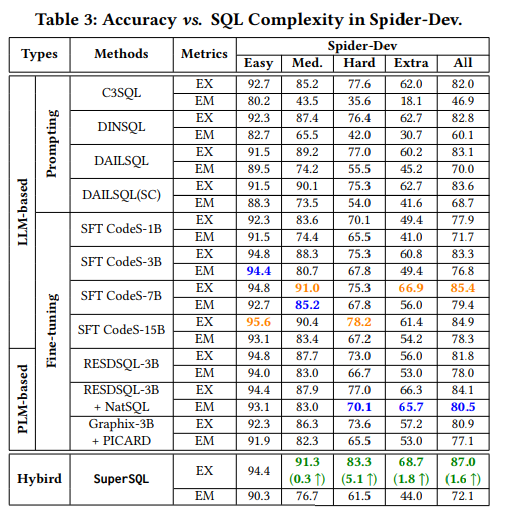
\includegraphics[width=0.5\textwidth]{img/dawn-nl2sql/acc-vs-complexity.png}
    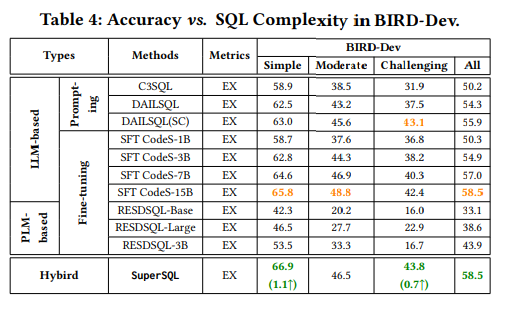
\includegraphics[width=0.5\textwidth]{img/dawn-nl2sql/acc-vs-complexity-bird.png}
    \caption{SQLの複雑度に対する精度}
    \label{fig:acc-vs-complexity}
\end{figure}

\begin{experiment}{実験結果から得られた発見}
\begin{itemize}
    \item ファインチューニングは精度向上のために重要である.
    \item サブクエリを含むSQLを生成する場合はLLMベースの手法がPLMベースの手法を上回る.
    \item 論理演算子が必要とされる場合は、LLMベースの手法がPLMベースの手法よりも良い性能を示す.
    \item JOINが必要な場合は、LLMベースの手法がPLMベースの手法よりも良い性能を示す. NatSQLを中間表現として使うことでJOINを予測する複雑度を低減して精度が良くなる.
    \item ORDER BYによるLLM/PLMベースの手法の性能差はデータセットにより異なる.
    \item QVTに関してはLLMとPLMの手法で明確な優劣はない.
    \item データベース数が多いドメインではそのデータでのファインチューニングが精度に大きく寄与する.
    \item 教師ありファインチューニングのあとでは、モデルのコーディング性能とSQL生成性能に大きな相関がある. よってコーディング性能が高いLLMを使うことが重要.
\end{itemize}
\end{experiment}

\begin{method}{SuperSQL}
    さまざまなNL2SQL手法を遺伝的アルゴリズムによって自動的に探索することで、SuperSQLという新たなNL2SQL手法を提案する.
    \begin{itemize}
        \item 設計空間: 前処理、プロンプト戦略、SQL生成戦略、後処理などのモジュールがある. 
        \item 上の設計空間を定義し、遺伝的アルゴリズムで探索することで、最適なNL2SQL手法を見つける.
        \item 遺伝的アルゴリズムによって発見された戦略: SuperSQLは以下のように構成される.
        \begin{itemize}
            \item 前処理: RESDSQLのスキーマリンキング、BRIDGE v2のDB Contents
            \item プロンプト生成: DAILSQLのFew-Shotモジュール
            \item SQL生成: OpenAIのGreedy Decoding
            \item 後処理: DAILSQLのSelf-Consistency
        \end{itemize}
        \item SuperSQLのSpider, BIRDでのEXは図\ref{fig:acc-vs-complexity}に示している. SpiderのMedium-Extraなどの難しいテストセット上でよい性能を示した.
    \end{itemize}
\end{method}

\section{感想}
\begin{kansou}
\begin{itemize}
  \item LLMをファインチューニングするときに同じドメインの(クエリ対象のテーブルが同じ)クエリを含んでいるのかが気になった. あまりそこには言及されていないがそれがあるかないかでファインチューニングの効果が変わるのではないかと思った.
  \item LLMベースの手法でもファインチューニングが効くのだということが分かった.
  \item 実験によってどの手法がどのような条件で有効なのかわかってきたのがよかった, 詳細な各手法についてくわしくないので調べたいと思った.
\end{itemize}
\end{kansou}

\bibliographystyle{jplain}
\bibliography{template.bib}

\end{document}